\documentclass[]{article}
\usepackage[german]{babel}
\usepackage{graphicx}
\usepackage{tabularx}
\usepackage[backend=bibtex, natbib=true]{biblatex}
\usepackage{listings}
\usepackage{tikz}

\lstset{%
	basicstyle=\ttfamily\scriptsize,        % Code font, Examples: \footnotesize, \ttfamily
	keywordstyle=\color{blue!80!black},     % Keywords font ('*' = uppercase)
	commentstyle=\color{gray},              % Comments font
	numbers=left,                           % Line nums position
	numberstyle=\tiny,                      % Line-numbers fonts
	stepnumber=1,                           % Step between two line-numbers
	numbersep=5pt,                          % How far are line-numbers from code
	backgroundcolor=\color{gray!10!white},  % Choose background color
	frame=none,                             % A frame around the code
	tabsize=2,                              % Default tab size
	captionpos=b,                           % Caption-position = bottom
	breaklines=true,                        % Automatic line breaking?
	breakatwhitespace=false,                % Automatic breaks only at whitespace?
	showspaces=false,                       % Dont make spaces visible
	showstringspaces=false                  %
	showtabs=false,                         % Dont make tabls visible
	columns=flexible,                       % Column format
	morekeywords={},                        % Specific keywords
	stringstyle=\color{green!50!black},%
}%

\bibliography{bibliography}
%opening
%Here you can enter your names and titleof your report
\title{Weekly Reports}
\author{Luftqualität in Innenräumen - Gruppe 1}

\begin{document}

\maketitle

\begin{table}[h!]
	\centering
	\begin{tabular}{|c|c|c|}
		\hline
		{\textbf{Name}}				&		{\textbf{Matrikel Nr.}} & {\textbf{Arbeitsaufwand (h)}} \\
		\hline
		Friedrich Just				&		1326699 				&		18,00\\
		\hline
		Stipe Knez					&		1269206 				&	19,00	\\
		\hline
		Lucas Merkert				&		1326709					&	20,00	\\
		\hline
		Achim Glaesmann				&		1309221					&	17,50	\\
		\hline
		Max-Rene Konieczka			&		1211092					&	18,00	\\
		\hline
		Can Cihan Nazlier			&		1179244					&	14,00	\\
		\hline
	\end{tabular}
	\caption{Arbeitsaufwand dieser Woche}
	\label{tab:worakload}
\end{table}



\section{Überblick}


\subsection{Friedrich Just}
Diese Woche wurden der Code für alle Sensoren  in ein Programm zusammengeführt. Danach wurde dieser Mikrocontroller in unser Zigbee-Netzwerk integriert. Nun werden die aktuellen Sensordaten an den Koordinator gesendet wie in Abbildung \ref{img:Messdaten} zu sehen ist. Eine Zeile steht für ein Paket mit Messungen aller 3 Sensoren.
An erster Stelle steht die Nummer des Endgerätes. Es folgen der Sensor SHT21 mit den Messwerten der Temperatur und der relativen Luftfeuchtigkeit. Danach stehen die Werte des SCD41 mit der Temperatur, der relativen Luftfeuchtigkeit und dem CO2-Wert. Als Letztes kommt der CSS811 mit dem eCO2 und dem TVOC. Alle Temperatur- und Luftfeuchtigkeitswerte müssen durch 100 geteilt werden, damit der richtige Wert als Gleitkommazahl heraus kommt.
\\\\
Bei dem CSS811 werden aus bisher noch nicht nachvollziehbaren Gründen falsche Werte an den Koordinator übertragen. Allerdings werden plausible Werte ausgegeben, wenn der Mikrocontroller direkt angeschlossen wird. (Siehe Abbildung \ref{img:CCS811_data}) Außerdem ist bei der Berechnung des SHT21 etwas falsch, da dies zu hohe Werte sind. Der SCD41 gibt hingegen plausible Werte aus, denn ähnliche Werte habe ich mit einem separaten Sensor gemessen. Die Messdaten wurden erhoben, während Frischluft durch das geöffnete Fenster eindringen konnte.
\begin{figure}[!h]
	\centering
	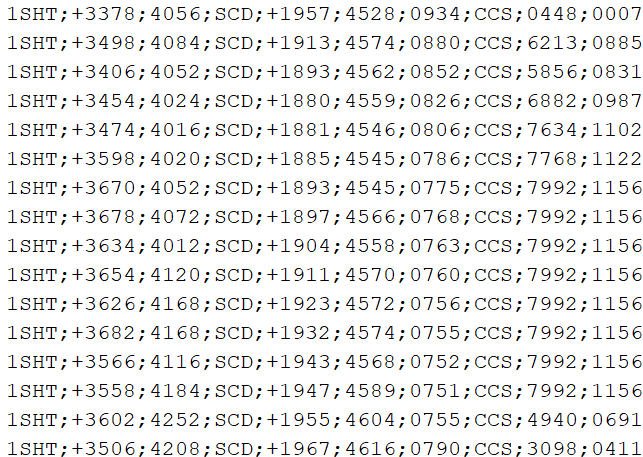
\includegraphics[scale=0.60]{images/Messdaten}
	\caption{Messdaten}
	\label{img:Messdaten}
\end{figure}

\begin{figure}[!h]
	\centering
	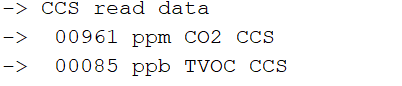
\includegraphics[scale=0.60]{images/CCS811_data}
	\caption{Messdaten CCS811}
	\label{img:CCS811_data}
\end{figure}





\subsection{Stipe Knez}
Vergangene Woche wurde sich dazu entschieden, das Format, in dem die Daten der ZigBee Module an das Backend geschickt werden, zu überarbeiten. Anstatt die Daten in Form von JSON Strings an das Backend zu schicken, sollten diese nun in Form von regulären Strings, bei denen die Werte mit einem Semikolon getrennt werden, geschickt werden. Diese Funktionalität konnten wir im Verlauf der Woche mit Hilfe eines entsprechenden Parsers erfolgreich im Backend implementieren. Als nächstes wurde begonnen sich dem Übertragen der Daten vom Back- in das Frontend und der Erstellung eines Dashboards mit Hilfe der D3.js Library zuzuwenden.
\subsection{Lucas Merkert}
Diese Woche wurde der CCS811 Sensor zum laufen gebracht. Hierbei haben wir uns mithilfe der Informationen von Dienstag einen geeigneten Zustandsautomaten wie in Abbildung \ref{img:Zustandsautomat} überlegt und diesen dann umgesetzt. Hierbei wurde der Sensor über die Adresse 0x5A angesprochen angesprochen. Im ersten Zustand wechselt der Sensor in den BOOT Modus damit ein Software-Reset durchgeführt werden kann und die Hardware ID überprüft werden kann. Danach wechselt der Sensor wieder in den APP Modus. In das MEAS\_MODE Register wird dann der Befehl geschrieben, dass der Sensor jede Sekunde misst. Zuletzt wird noch im Status Register überprüft ob Daten bereit liegen und diese werden dann ausgelesen. Dies geschieht in einem Zyklus von einer Sekunde.

\begin{figure}[h]
	\centering
	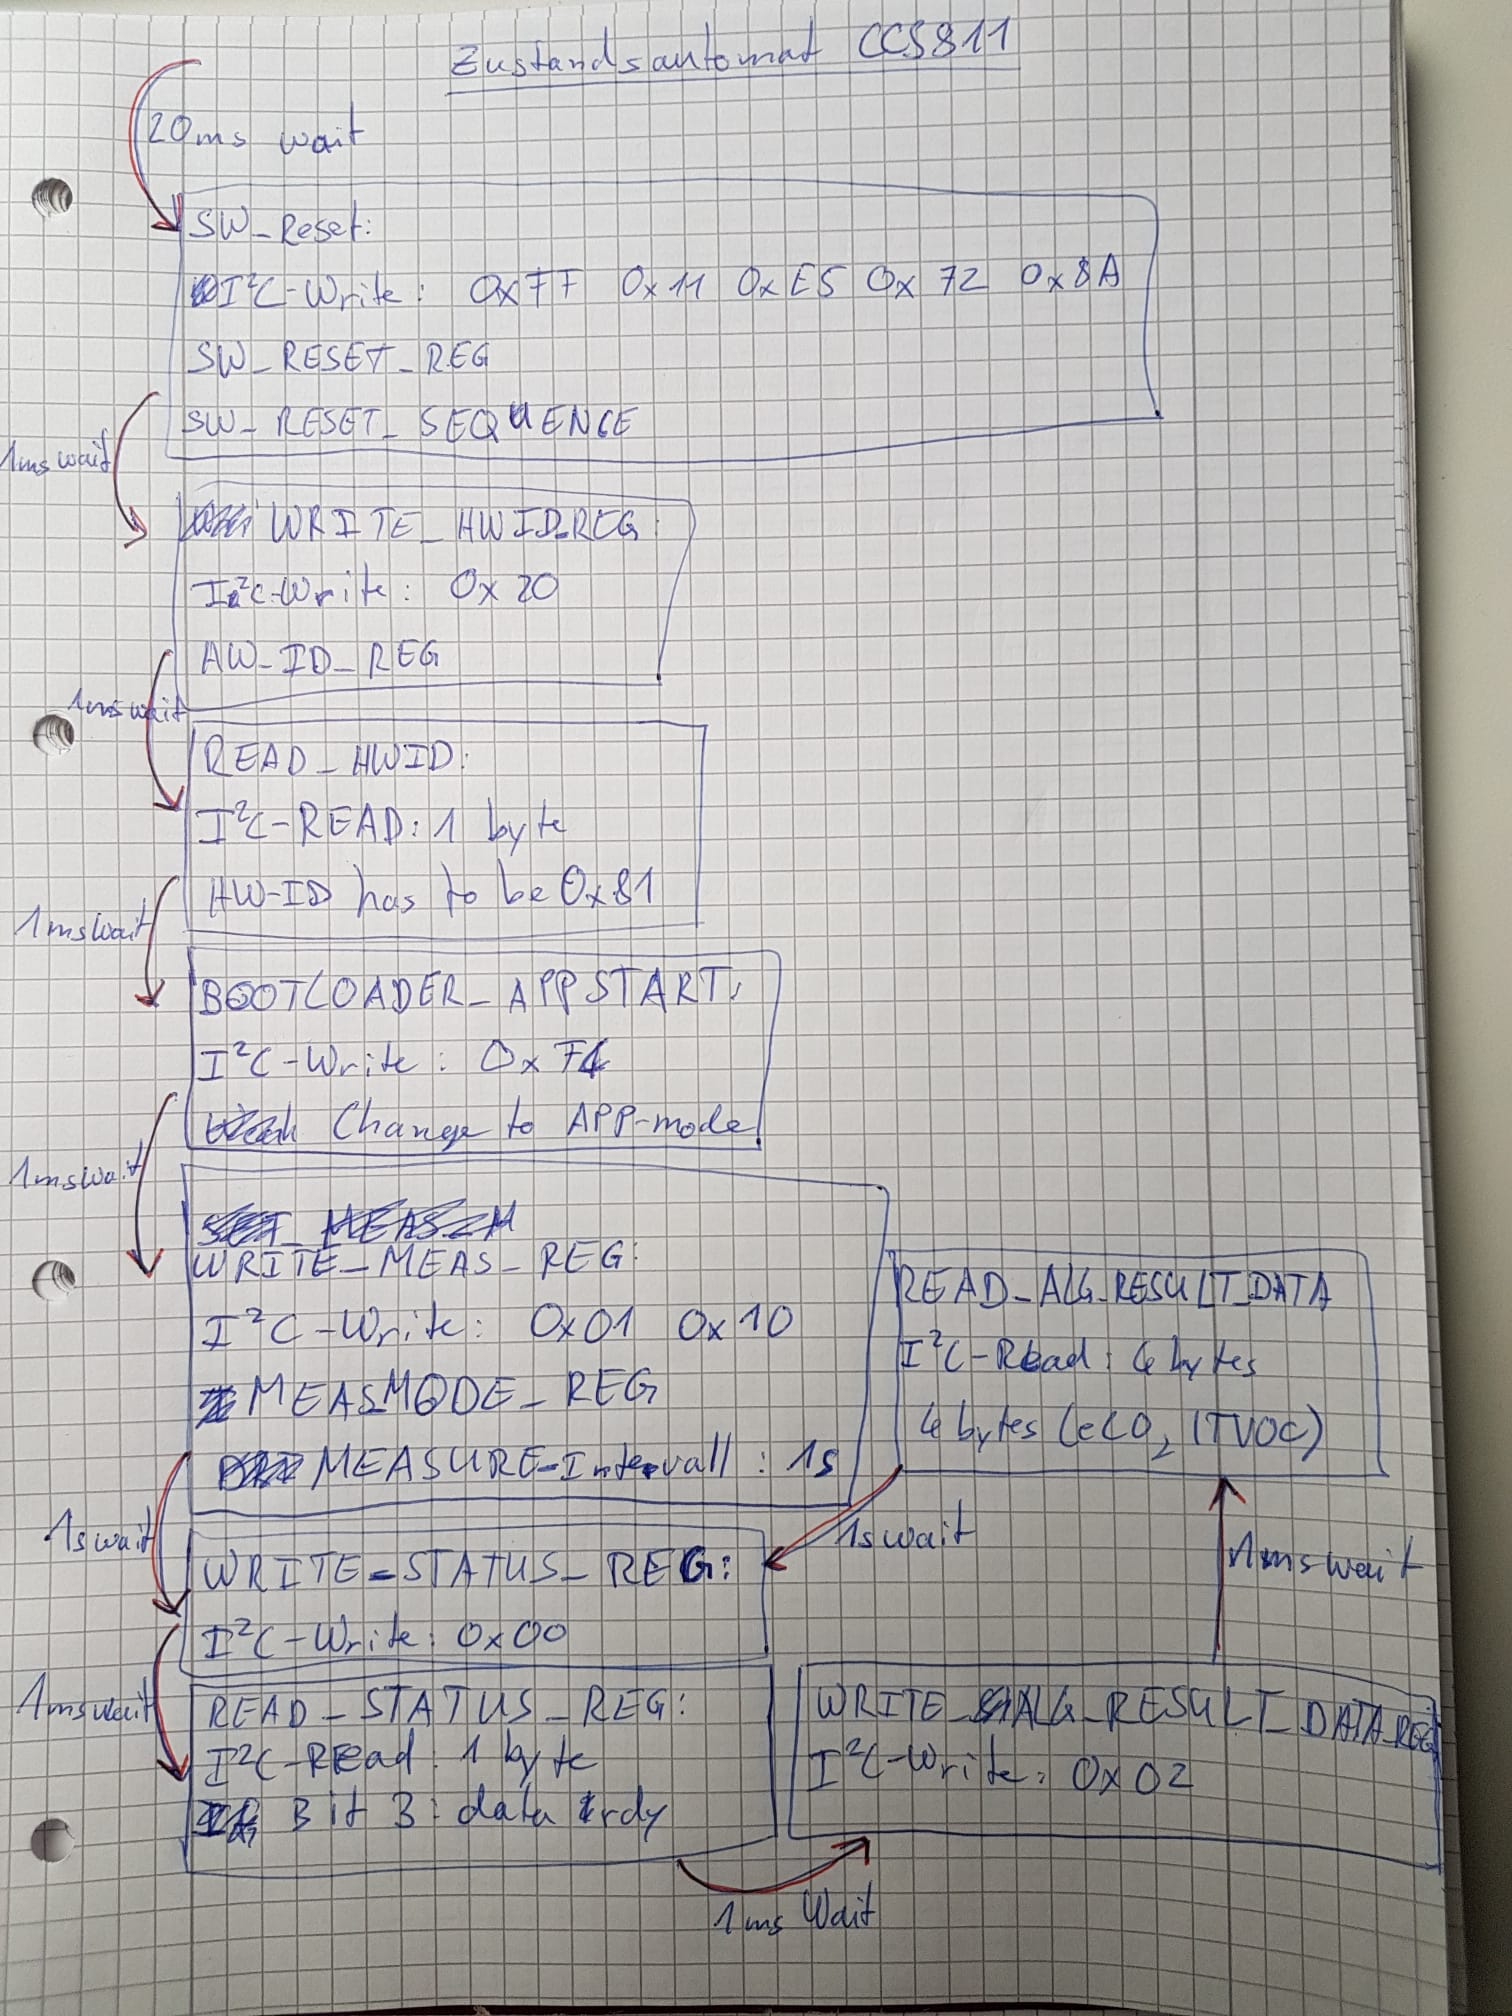
\includegraphics[scale=0.20]{images/zustandsautomat_ccs811}
	\caption{Zustandsautomat CCS811}
	\label{img:Zustandsautomat}
\end{figure}

\subsection{Achim Glaesmann}
Diese Woche wurde dazu verwendet die von den Verschiedenen Teammitgliedern übernommenen Aufgaben bezüglich der Auslesung des Sensors und der Übertragung der Daten über das Zigbee Protokoll zusammenzuführen. Zunächst wurde sich persönlich getroffen, um in der Gruppe Probleme beim Auslesen des CCS811 und dem Aufbau des Funknetzes zu lösen. Nach testen des Sensors am Arduino und dem Übertragen der Programmlogik der anderen Sensoren auf den AVR-Chip, war es trotz mehrfachen Prüfen des Codes nicht möglich eine I2C-Kommunikation zum CCS aufzubauen. Selbst nach ausführlichem Testen und mehrmaligen umschreiben einzelner Softwarekomponenten, konnte das Problem nicht behoben werden. Es stellte sich heraus, das es kein softwareseitiges Problem war. Nach austauschen des Funkmoduls war es möglich eine Kommunikation zwischen Sensor und Mikrokontroller zu etablieren. Der Mikrokontroller wurde markiert und wird nochmal überprüft. Nachdem sowohl das Auslesen des CSS811, als auch Aufbau des Funknetzwerkes realisiert wurden, war es nötig die einzelnen Softwarelösungen für die Sensoren und das Netzwerk zu kombinieren. Dies wurde erfolgreich erledigt. Als nächste Aufgabe ist es nun nötig, die Übermittelten Daten an das Backend der Desktop-Applikation zu übermitteln.

\subsection{Max-Rene Konieczka}
Im Verlauf der letzten Woche wurde daran gearbeitet, Strings über Atmel Studio zu versenden und diese anschließend in unserer Datenbank anzeigen zu lassen. Nachdem dies gelungen ist, wurde angefangen sich mit dem Dashboard auseinanderzusetzen. Es wurde überlegt, die D3.js Library von Javascript~\cite{D3JS} zu verwenden. Mit D3.js ist es möglich einfache Formen bis hin zu detaillierten Diagrammen zu erstellen.
Die Daten der Sensoren sollen nun mithilfe der Axis API von D3 in einem Koordinatensystem dargestellt werden. 
\subsection{Can Cihan Nazlier}
Durchgehen der Dokumentation von d3js. Websockets vorbereiten, sodass server side events gesendet werden können. Warum Websockets?
Antwort: das frontend und das backend laufen als zwei seperate anwendungen und müssen sich untereinander austauschen. Das geschieht eigentlich über http. Das Problem jedoch ist,
für http muss der Client dem Server request schicken um Daten zu empfangen. Da die Sensordaten im Backend ankommen und wenn die Kommunikation nur mittels http geschieht, so müsste der client alle 10 minuten eine Anfrage an den Server senden und es könnte durchaus dazu kommen , dass wir einzelne Messungen verpassen. Deshalb ist es wichtig, dass der server dem Client Daten sendet sobald welche da sind. Dazu wurde nun die Grundlage gelegt. 


\printbibliography
%----------------------------------------------------------------------------
% Bibliography
%----------------------------------------------------------------------------	

\end{document}
